\documentclass{beamer}
\usepackage{amsfonts,amsmath,oldgerm}
\usepackage{listings}
\usepackage{xcolor}
\usetheme{sintef43}
\AtBeginSection[]{}

% Set frame title font size to normal
\setbeamerfont{frametitle}{size=\normalsize}

% Shift frame title position up
\setbeamertemplate{frametitle}{
  \vspace{-0.5cm}
  \begin{beamercolorbox}[wd=\paperwidth,ht=1.2em,dp=0.5em,center]{frametitle}
    \usebeamerfont{frametitle}\insertframetitle
  \end{beamercolorbox}
}

% Reduce overall font sizes for better fit
\setbeamerfont{normal text}{size=\footnotesize}
\setbeamerfont{block title}{size=\footnotesize}
\setbeamerfont{block body}{size=\footnotesize}
\setbeamerfont{itemize/enumerate body}{size=\footnotesize}
\setbeamerfont{itemize/enumerate subbody}{size=\footnotesize}
\setbeamerfont{itemize/enumerate subsubbody}{size=\footnotesize}

\usefonttheme[onlymath]{serif}
\usepackage{amsmath,amssymb,mathtools}
\usefonttheme{professionalfonts}

% Configure listings for Python code
\lstset{
    language=Python,
    basicstyle=\ttfamily\footnotesize,
    keywordstyle=\color{blue},
    commentstyle=\color{gray},
    stringstyle=\color{red},
    showstringspaces=false,
    breaklines=true,
    frame=single,
    backgroundcolor=\color{gray!10}
}

\usepackage{hyperref}
\hypersetup{
    pdfauthor={Research Team, Bioinformatics Laboratory},
    pdftitle={sxSNF: Single-cell Multi-modal Fusion Analysis Pipeline},
    pdfsubject={Computational Biology Symposium},
    pdfkeywords={single-cell, multi-modal, SNF, graph neural networks, bioinformatics},
    pdfcreator={XeLaTeX},
    pdfproducer={XeLaTeX},
    unicode=true
}


% Use SINTEF theme's sintefyellow plus bold for highlighting
\newcommand{\hrefcol}[2]{\textcolor{sintefyellow}{\textbf{\href{#1}{#2}}}}

% Remove automatic subtitles in SINTEF theme
\makeatletter
\def\beamer@checkframetitle{\@ifnextchar\bgroup\beamer@inlineframetitle{}}
\makeatother

\title{sxSNF: A Novel Single-Cell Multi-Modal Data Integration Method Combining Similarity Network Fusion and Deep Graph Learning}

\author{%
    Li C. Xia
}
\institute{\small Department of Statistics and Financial Mathematics, School of Mathematics, South China University of Technology}

% Redefine the title page to include institute with full width title
\makeatletter
\setbeamertemplate{title page}{%
  \vskip0pt plus 0.3filll%
  \vspace{2mm}
  \begin{beamercolorbox}[wd=\textwidth,sep=8pt,leftskip=0pt,rightskip=0pt]{title}%
    {\usebeamerfont{title}\inserttitle}
    \vspace{5ex}
    
    {\usebeamerfont{author}\usebeamercolor[fg]{author}\textbf{\insertauthor}}
    \vspace{0.5ex}
    
    {\usebeamerfont{institute}\usebeamercolor[fg]{institute}\insertinstitute}
    \vspace{0.5ex}
    
    {\usebeamerfont{date}\usebeamercolor[fg]{date}\insertdate}
  \end{beamercolorbox}
}
\makeatother

\date{APBC 2025\\ The 23rd Asia Pacific Bioinformatics Conference \\ September 21, 2025 | Nanjing, China}

\begin{document}
\maketitle

\section{Introduction}



\begin{frame}{Single Cell Multi-Modal Integration}

\begin{columns}[T]
\begin{column}{0.7\textwidth}
\textbf{Challenges:}

\begin{itemize}
\item \scriptsize \textbf{Cell Group Connection Variability}: Cell connections vary in dynamics, resulting in shifted group representation
\item \scriptsize \textbf{Limited Complementary Leveraging}: Previous methods not leveraging modality complementary information
\item \scriptsize \textbf{Batch Effects}: Modality specific distortions
\end{itemize}

\vspace{0.1cm}

\textbf{Our Proposed Algorithm (sxSNF):}

\begin{itemize}
\item \scriptsize \textcolor{sintefyellow}{\textbf{Similarity Network Fusion (SNF)}}: Initially in ref. [1], align complementary similarities through soft mutual diffusive process
\item \scriptsize \textbf{Dual Graph Representation}: Preserve modality-specific structures during the diffusion
\item \scriptsize \textbf{Network-based Representation Learning}: Not prone to batch effects
\end{itemize}
\end{column}

\begin{column}{0.3\textwidth}
\vspace{0pt}
\centering
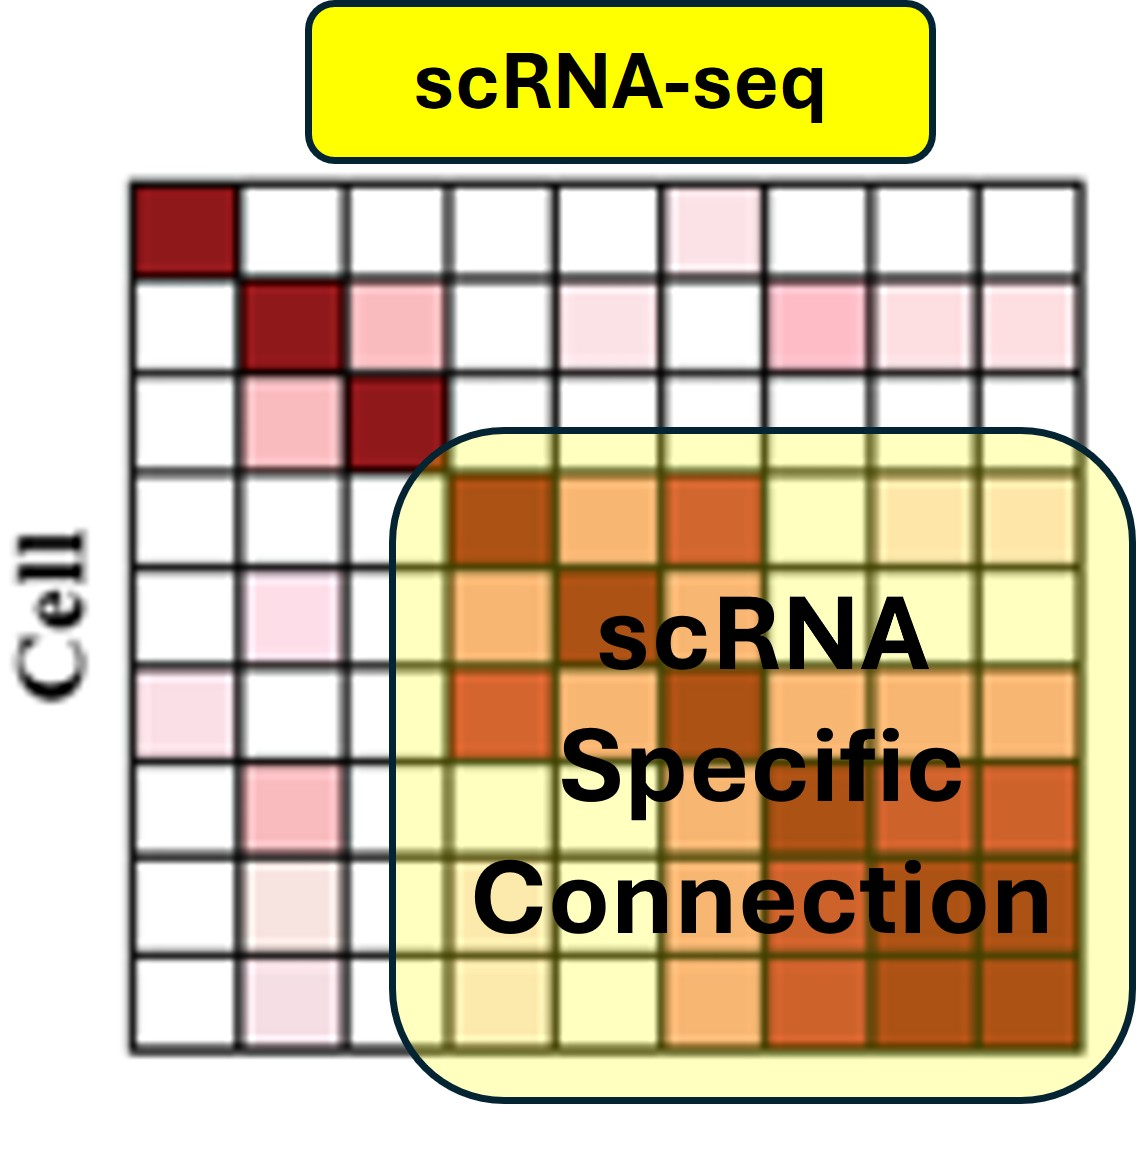
\includegraphics[width=0.95\textwidth,height=3.2cm,keepaspectratio]{./sxSNF_figure/Fig1a.jpg}

\vspace{0.1cm}

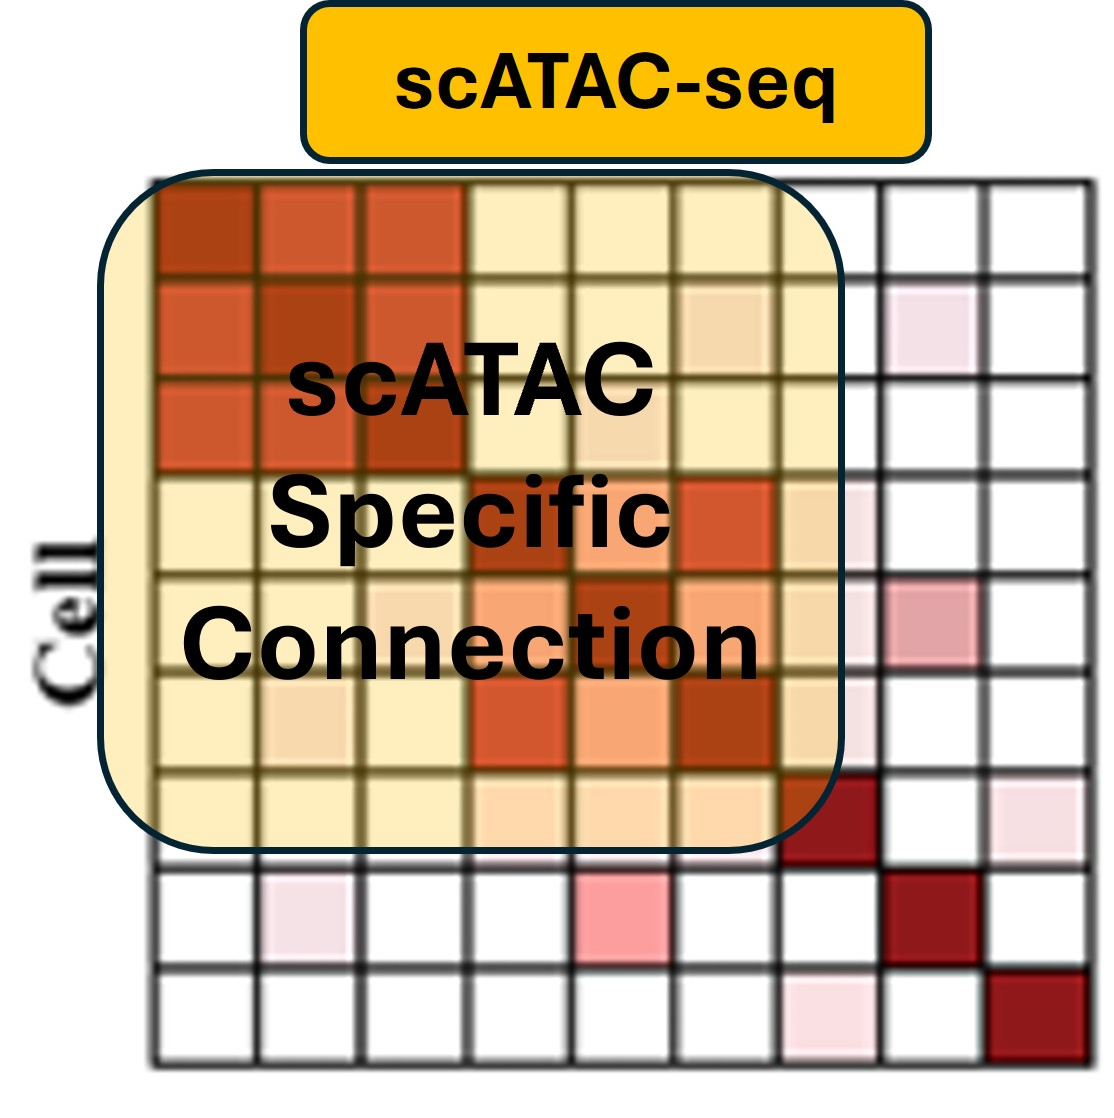
\includegraphics[width=0.95\textwidth,height=3.2cm,keepaspectratio]{./sxSNF_figure/Fig1b.jpg}
\end{column}
\end{columns}

\end{frame}






\begin{frame}{Methods of Fusion}
\begin{itemize}
\item \textbf{Simple Concatenation}
\[
X_{combined} = [X^{(1)}, X^{(2)}, \ldots, X^{(M)}]
\]
\vspace{-2ex}
  \begin{itemize}
  \item \scriptsize Loses intrinsic structure of each modality; Suffers from scale differences; ...
  \end{itemize}

\item \textbf{Weighted Integration}
\[
X_{fused} = \sum_{m=1}^{M} \alpha_m X^{(m)}, \quad \sum_{m=1}^{M} \alpha_m = 1
\]
\vspace{-2ex}
  \begin{itemize}
  \item \scriptsize Difficult to determine optimal weights; Static weighting ignores modal-specific structure; ...
  \end{itemize}

\item \textcolor{sintefyellow}{\textbf{Our Idea: bring in SNF Fusion}}
\[
P^{(m)}(t+1)= S^{(m)} \frac{\sum_{k \neq m} P^{(k)}(t)}{M-1} (S^{(m)})^T
\]
\vspace{-2ex}
  \begin{itemize}
  \item \scriptsize $P^{(m)}$: cross-modal similarity matrix ; $S^{(m)}$: modality-specific similarity matrix; $M$ total modalities.
  \item \scriptsize \textbf{Core Idea}: SNF enables information flow in fusion while retaining local structures
  \end{itemize}
\end{itemize}
\end{frame}

\section{Methods}



\begin{frame}{sxSNF: SNF-based Cross-modal Graph Fusion}
\vspace{0.1cm}
\centering
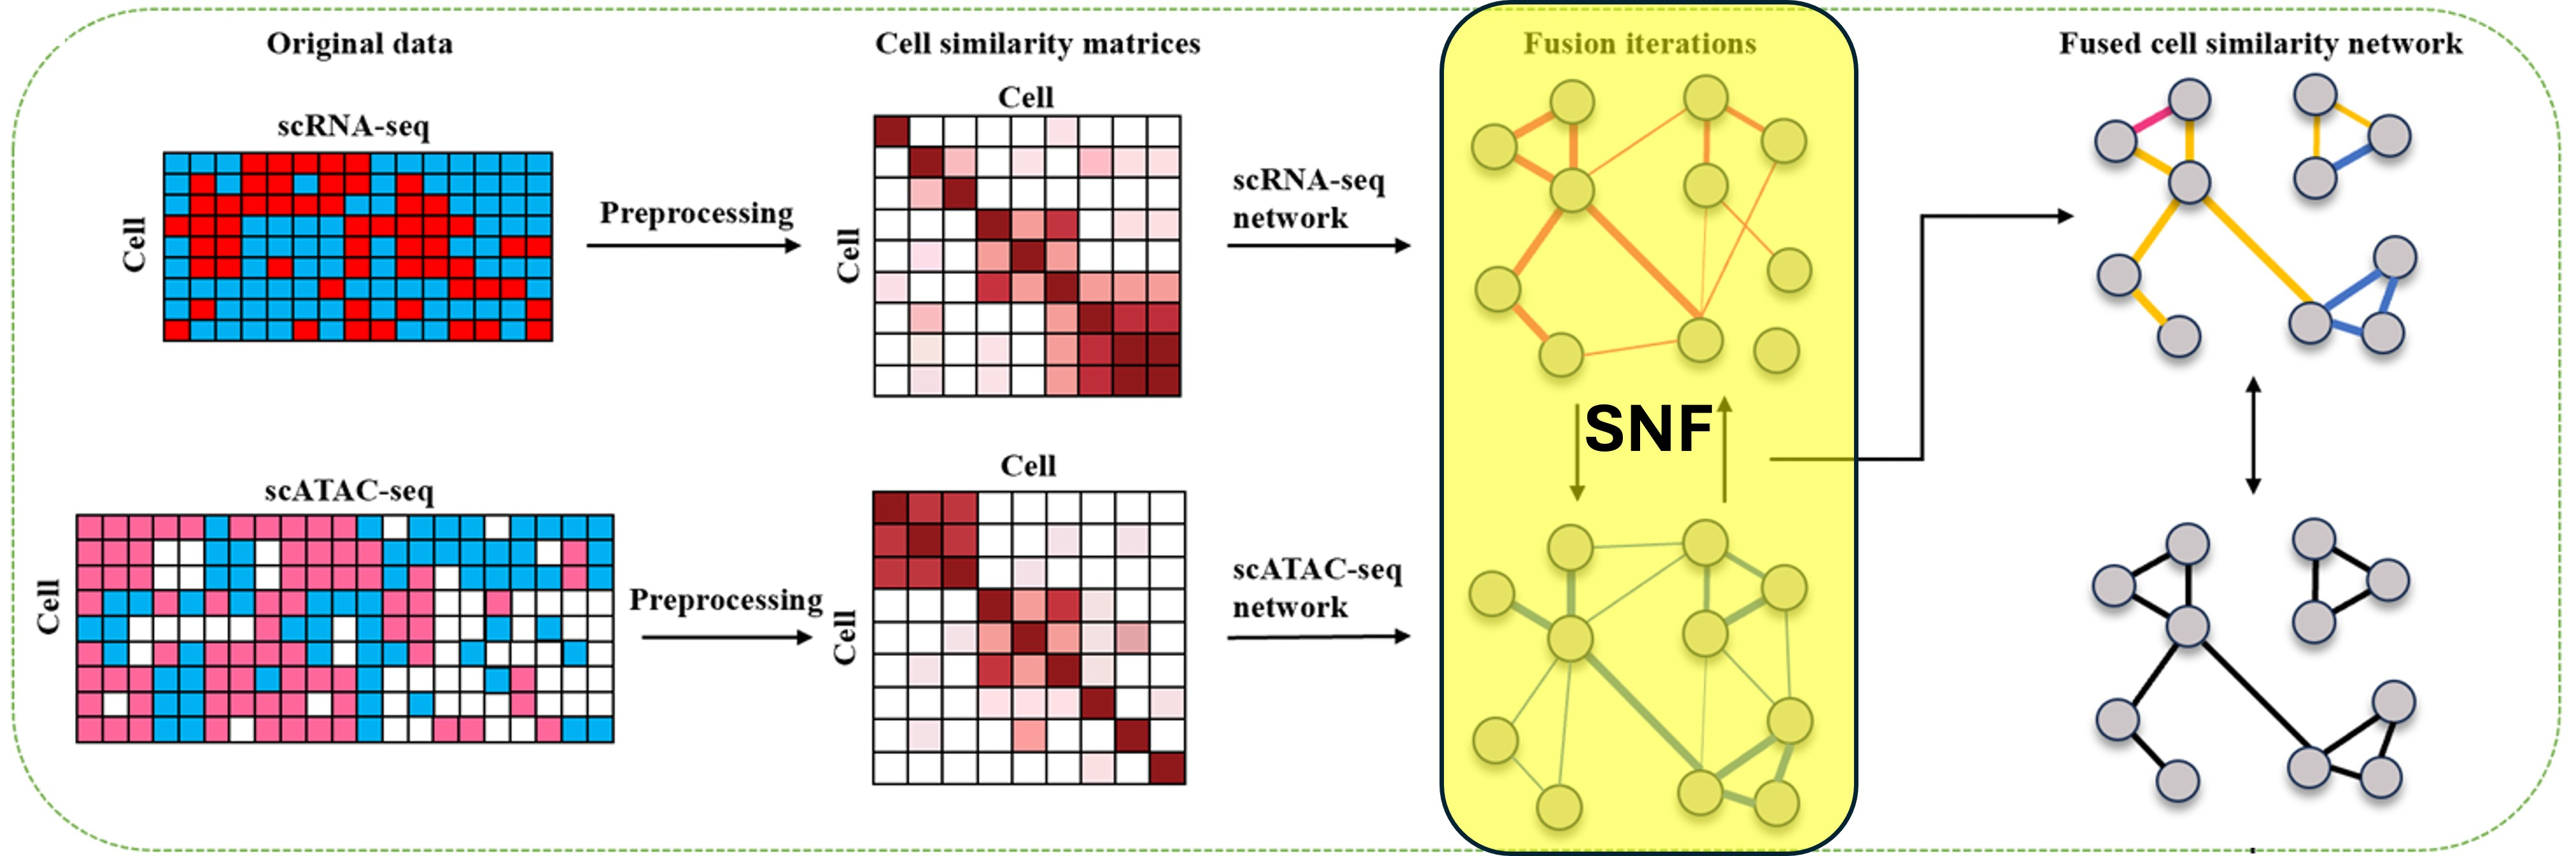
\includegraphics[width=1.0\textwidth,height=7cm,keepaspectratio]{./sxSNF_figure/Fig3a.jpg}

\vspace{0.1cm}

\scriptsize
\begin{itemize}
  \item Preprocess modal specific similarity matrices (e.g. scRNA-seq / scATAC-seq)
  \item Build modality-specific cell connection graphs (KNN)
  \item Apply SNF to iteratively exchange neighborhood information between modals
  \item Output a modal fused cell similarity network
\end{itemize}

\end{frame}
\begin{frame}{sxSNF: GNN Representation and Clustering}

\centering
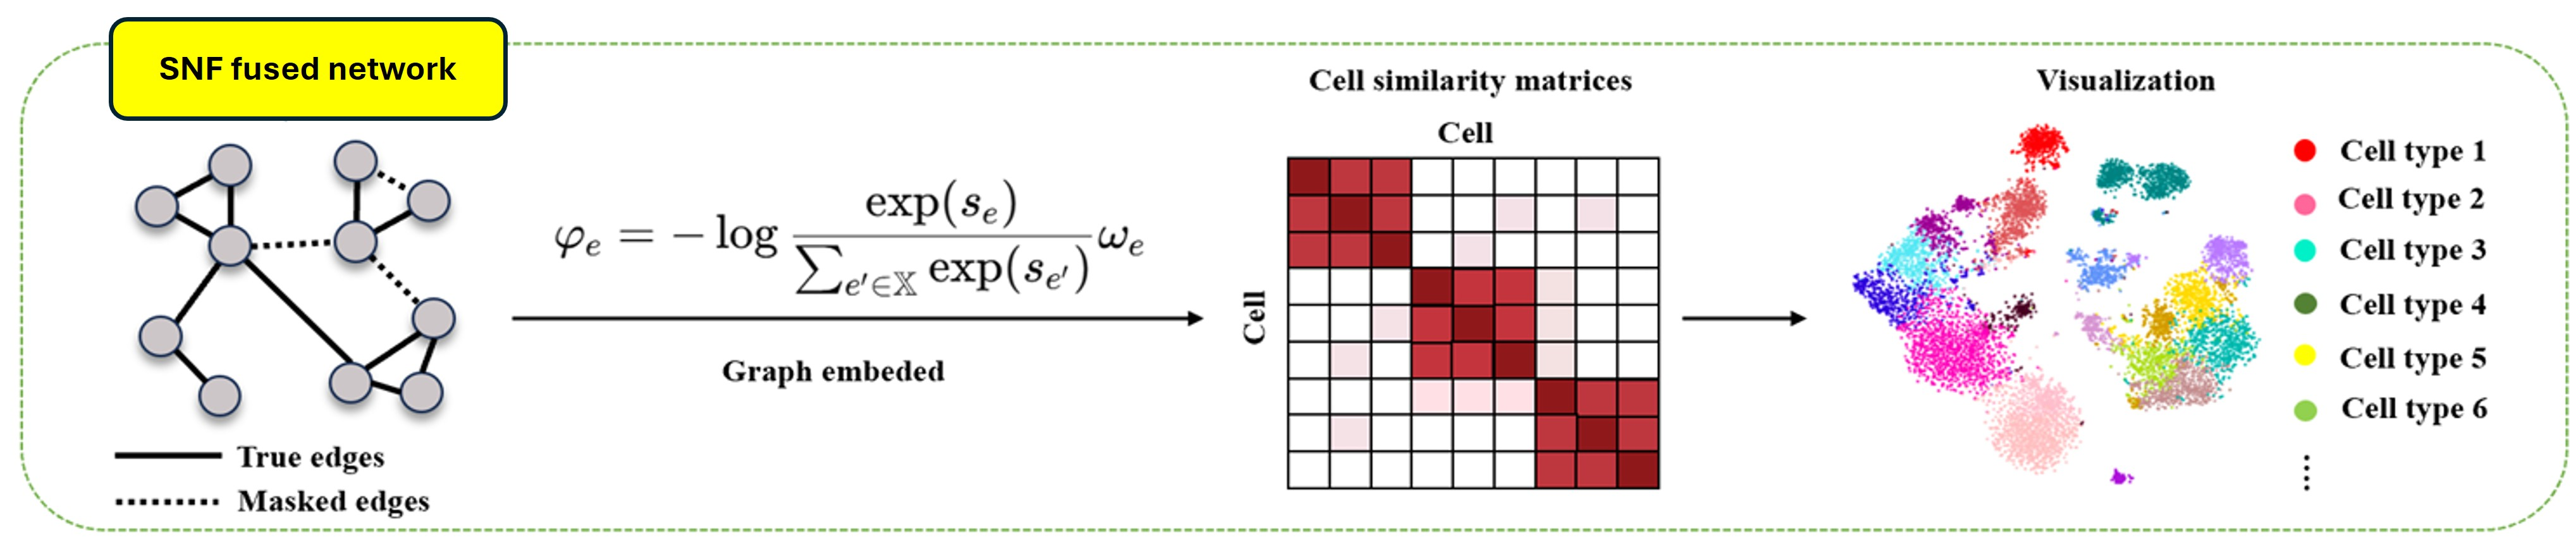
\includegraphics[width=1.0\textwidth,height=7cm,keepaspectratio]{./sxSNF_figure/Fig3b.jpg}

\vspace{0.1cm}

\scriptsize
\begin{itemize}
  \item Use each cell's adjacency vector from the SNF fused network as initial features
  \item Train GNN on the fused graph with masked-edge prediction
  \item Obtain low-dimensional embeddings of the fused cell characteristics
  \item Recompute similarity → clustering → UMAP visualization
\end{itemize}

\end{frame}







\begin{frame}{sxSNF Algorithm (scRNA + scATAC)}

\footnotesize
\textbf{Step 1: Modality-specific Preprocessing}

\textbf{scRNA-seq preprocessing:}
\[
X^{RNA}_{i,j} = \log\left(1 + \frac{X^{RNA}_{i,j} \times 10^4}{\sum_{g,j} X^{RNA}_{g,j}}\right)
\]

\textbf{scATAC-seq preprocessing:}
\[
X^{ATAC}_{i,j} = \text{TF-IDF}(X^{ATAC}_{peaks}) = \log\left(1 + \frac{tX^{ATAC}_{i,j} \times \log(\frac{N}{dX^{ATAC}_j})}{||tX^{ATAC}_i||_2}\right)
\]

\vspace{0.1cm}

\textbf{Step 2: Similarity Network Construction}

For each modality $m$, construct cell similarity network:
\[
S^{(m)}_{ij}=P^{(m)}_{ij}(0)={\rm KNN}_{k}\left(\exp\left(-\frac{d^2_{cos}(x^{(m)}_i, x^{(m)}_j)}{\tau^2}\right)\right)
\]

where $d_{cos}(.)$ is cosine distance, $\tau$ controls neighborhood size, $k$ is number of nearest neighbours.
\end{frame}

\begin{frame}{sxSNF Algorithm (cont'd)}

\footnotesize
\textbf{Step 3: SNF Cross-modal Diffusion Process}

\textbf{Two-modal diffusion}:
\[
P^{(m)}(t+1) = S^{(m)} \times P^{(k)}(t) \times (S^{(m)})^T
\]

\textbf{Convergence}: Iterate until $||P^{(m)}(t+1) - P^{(m)}(t)||_F < \epsilon$

\vspace{0.1cm}

\textbf{Step 4: Train GNN (self-supervised with masked edge prediction):}
\[
\mathbf{h}_i^{(l+1)} = \sigma\!\left(\sum_{j\in\mathcal{N}(i)} \alpha_{ij} \mathbf{W}^{(l)} \mathbf{h}_j^{(l)}\right)
\]

\textbf{with objective}:
\[
\mathcal{L}_i = -\sum_{j \in \mathcal{N}(i)} \log \frac{\exp(\mathbf{h}_i^\top\mathbf{h}_j)}{\sum_{j'} \exp(\mathbf{h}_i^\top\mathbf{h}_{j'})}
\]

\textbf{Symbol definitions:}

\scriptsize
- $\mathbf{x}_i$: input feature of cell $i$; $\mathbf{h}_i$: hidden representation; $\alpha_{ij}$: edge weight; $\mathbf{W}^{(l)}$: weight matrix;  $\mathcal{N}(i)$: neighbor set; $E,\mathcal{V}$: edge/node sets
\end{frame}














\section{Experimental Design}

\begin{frame}{Datasets and Evaluation}

\textbf{Benchmark Datasets}:

\begin{table}[h]
\centering
\scriptsize
\begin{tabular}{|l|l|c|l|c|}
\hline
\rule{0pt}{3ex}\textbf{Dataset} & \textbf{Platform} & \textbf{Cells} & \textbf{Modalities} & \textbf{Cell Types}\rule[-1.5ex]{0pt}{0pt} \\
\hline
\rule{0pt}{3ex}\textbf{PBMC-10x} & 10X Genomics & 11,909 & scRNA+scATAC & 19 immune\rule[-1.5ex]{0pt}{0pt} \\
\hline
\rule{0pt}{3ex}\textbf{SHARE-seq} & SHARE-seq & 34,774 & scRNA+scATAC & 20 skin\rule[-1.5ex]{0pt}{0pt} \\
\hline 
\rule{0pt}{3ex}\textbf{SNARE-seq} & SNARE-seq & 15,390 & scRNA+scATAC & 13 brain\rule[-1.5ex]{0pt}{0pt} \\
\hline
\end{tabular}
\end{table}

\textbf{Evaluation Methods}:

\begin{itemize}
\item \textbf{Clustering Quality}: ARI, NMI, AMI
\item \textbf{Biological Validation}: Marker gene enrichment analysis
\item \textbf{Model Interpretability}: Low-dimension visualization by TSNE and UMAP
\end{itemize}
\end{frame}

\begin{frame}{Benchmark Results (PBMC-10x)}

\vspace{-1ex}
\begin{table}[h]
\centering
\scriptsize
\begin{tabular}{|l|c|c|c|c|c|c|c|}
\hline
\rule{0pt}{3ex}\textbf{Methods} & \textbf{sxSNF} & \textbf{SIMBA} & \textbf{scMIC} & \textbf{SNF+scMIC} & \textbf{Guanlab} & \textbf{DCCA}\rule[-1.5ex]{0pt}{0pt} \\
\hline
\rule{0pt}{3ex}\textbf{ARI} & \textcolor{sintefyellow}{\textbf{0.5584}} & 0.4854 & 0.1142 & 0.3523 & 0.2683 & 0.3375\rule[-1.5ex]{0pt}{0pt} \\
\hline
\rule{0pt}{3ex}\textbf{NMI} & \textcolor{sintefyellow}{\textbf{0.7274}} & 0.6839 & 0.2841 & 0.5732 & 0.5164 & 0.5798\rule[-1.5ex]{0pt}{0pt} \\
\hline
\rule{0pt}{3ex}\textbf{AMI} & \textcolor{sintefyellow}{\textbf{0.7260}} & 0.6822 & 0.2802 & 0.5710 & 0.5140 & 0.5777\rule[-1.5ex]{0pt}{0pt} \\
\hline
\end{tabular}
\end{table}

\vspace{0.1cm}

\scriptsize
\textbf{Method Descriptions}:
\begin{itemize}
    \item \scriptsize \textbf{SIMBA} [2]: Contrastive learning for multimodal integration (Chen et al., Nature Methods, 2024)
    \item \scriptsize \textbf{scMIC} [3]: Mutual information maximization approach (Zhan et al., IEEE JBHI, 2023)
    \item \scriptsize \textbf{SNF+scMIC}: Hybrid of SNF and scMIC strategies (An extension of the model scMIC by SNF)
    \item \scriptsize \textbf{Guanlab-dengkw} [4]: Sparse regularization and graph learning (Hu et al., Nature Methods, 2024)
    \item \scriptsize \textbf{DCCA} [5]: Deep canonical correlation analysis (Zuo et al., Bioinformatics, 2021)
\end{itemize}

\end{frame}
  
\begin{frame}{T-SNE Visualization (SNARE-seq)}
\begin{center}
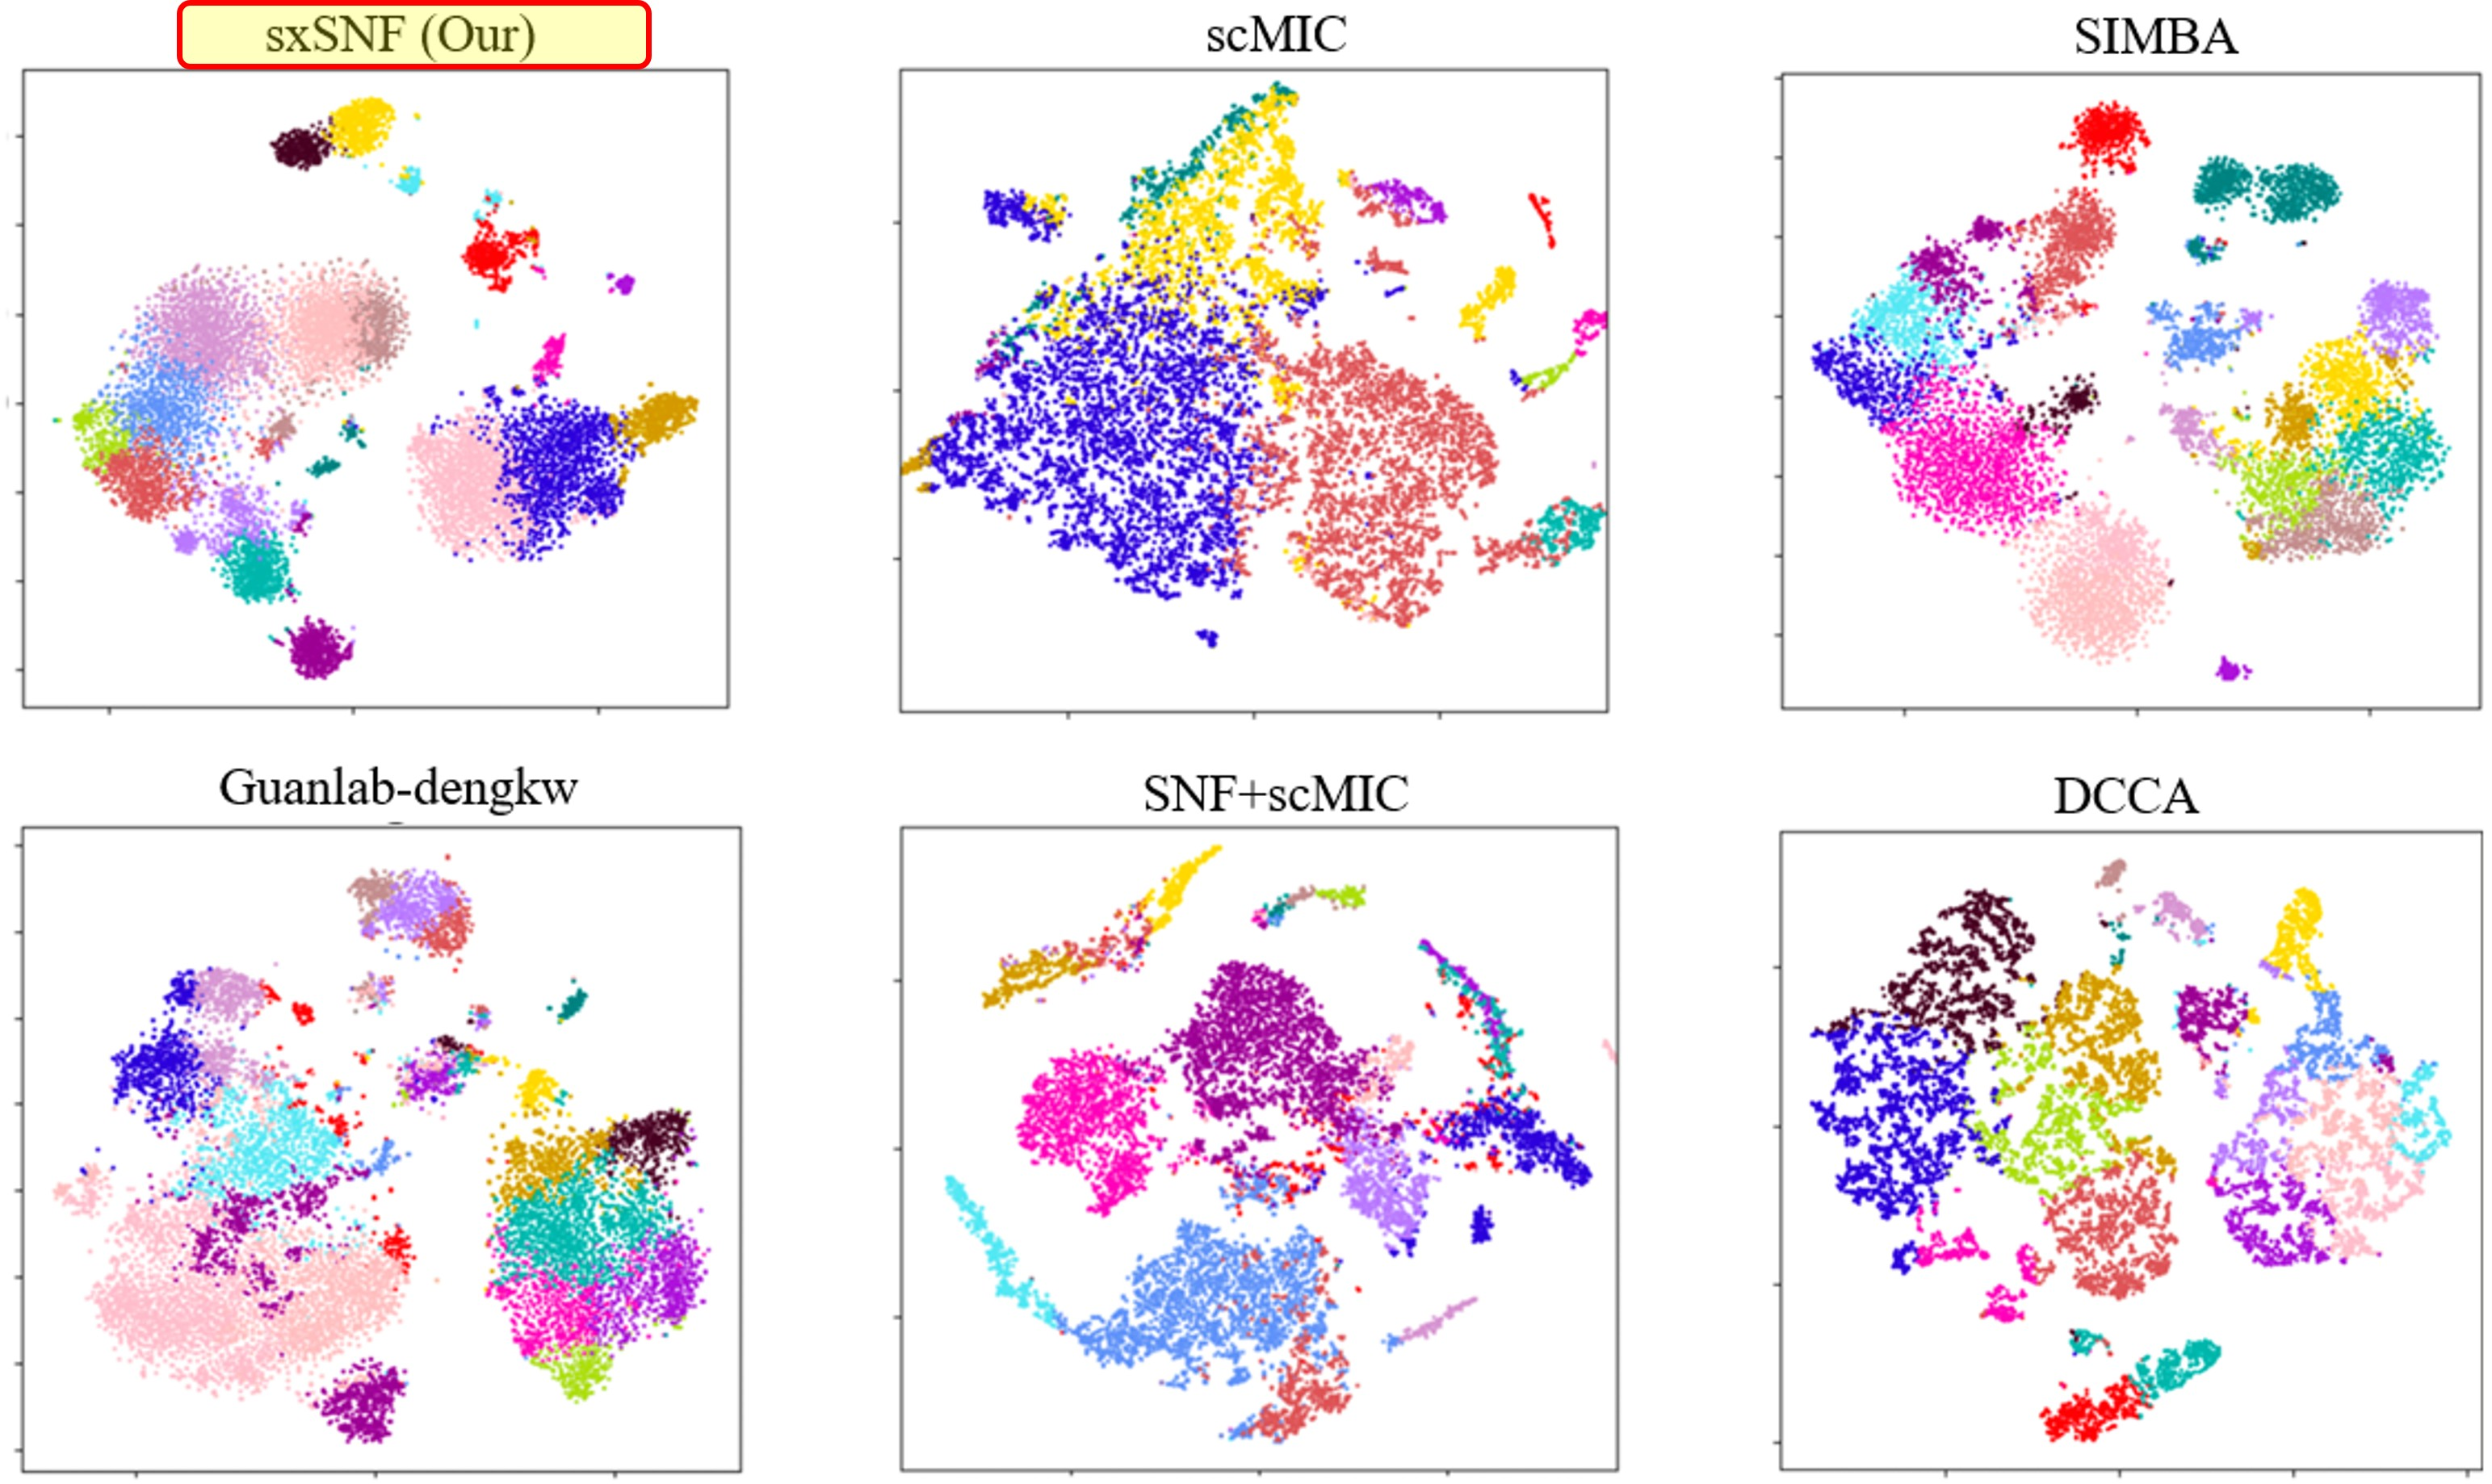
\includegraphics[width=1.0\textwidth,height=8cm,keepaspectratio]{./sxSNF_figure/Fig4.jpg}
\end{center}
\end{frame}

\begin{frame}{UMAP Visualization (SHARE-seq)}
\vspace{0.1cm}
\centering
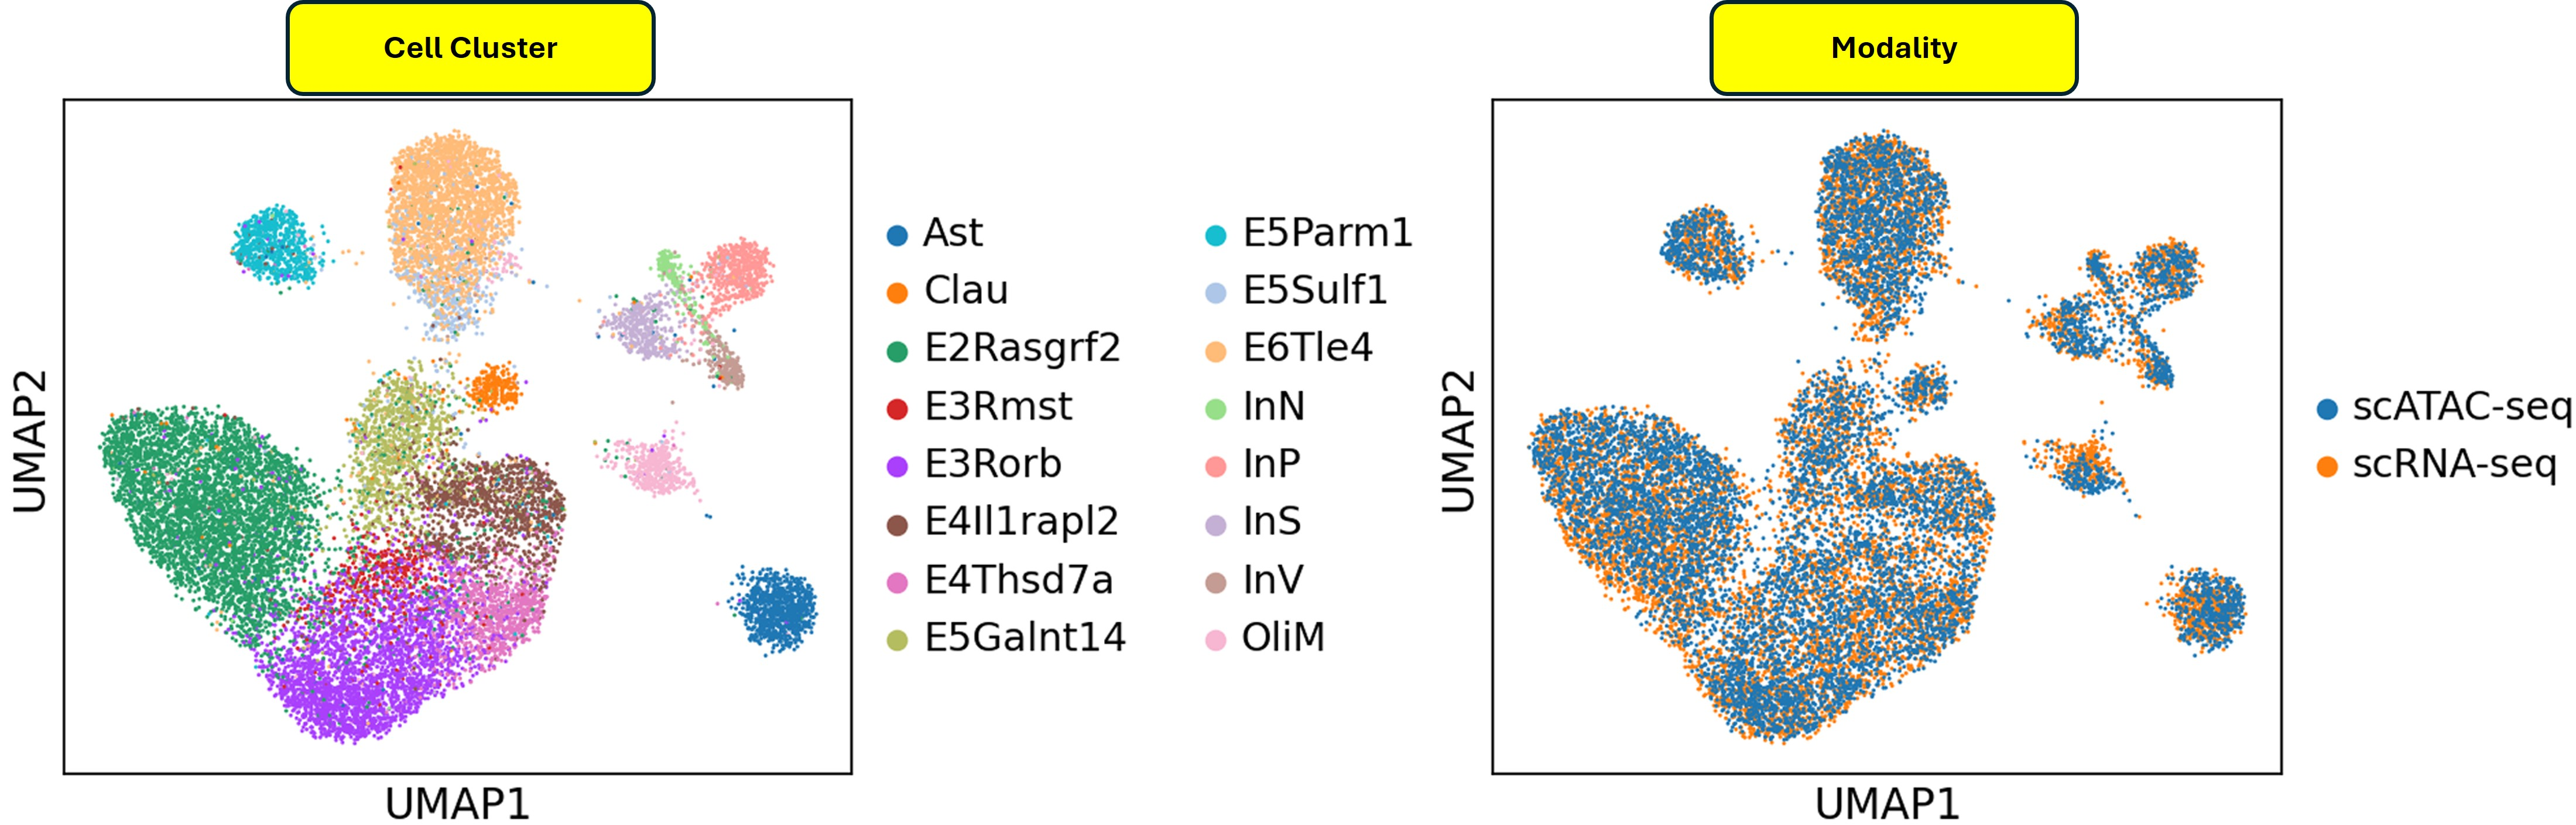
\includegraphics[width=1.0\textwidth,height=7cm,keepaspectratio]{./sxSNF_figure/Fig5.jpg}

\vspace{0.1cm}

\begin{center}
\begin{itemize}
  \item \textbf{Clear separation of cell types (left panel)}  
  \begin{itemize}\footnotesize
      \item Joint embedding yields well-defined clusters with sharp boundaries
  \end{itemize}

  \item \textbf{Effective cross-modal alignment (right panel)}  
  \begin{itemize}\footnotesize
      \item scRNA-seq (orange) and scATAC-seq (blue) cells are well mixed within clusters  
      \item Indicates successful integration of complementary modalities
  \end{itemize}
\end{itemize}
\end{center}

\end{frame}



\begin{frame}{Marker Gene Expression (SNARE-seq)}

\centering
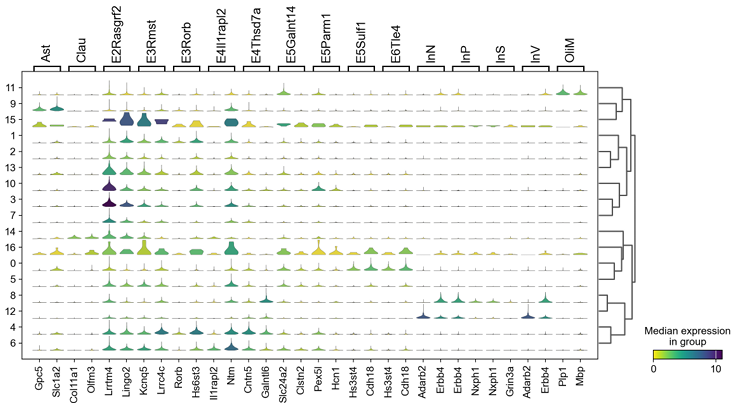
\includegraphics[width=1.0\textwidth,height=6cm,keepaspectratio]{./sxSNF_figure/figure_6.png}

\begin{itemize}\scriptsize
    \item Distinct marker gene expression patterns validate the identified cell clusters
    \item Hierarchical clustering reveals lineage relationships among cell types
\end{itemize}

\end{frame}



\begin{frame}{Summary}

\normalsize
\begin{itemize}
\item We developed \textcolor{sintefyellow}{\textbf{sxSNF}} - a \textcolor{sintefyellow}{\textbf{novel}} tool combines Similarity Network Fusion (SNF) with Graph Neural Networks for single-cell multi-modal data integration
\item It \textcolor{sintefyellow}{\textbf{preserves modality-specific structures}} while enabling \textcolor{sintefyellow}{\textbf{cross-modal information flow}} through iterative neighborhood exchange
\item Its \textcolor{sintefyellow}{\textbf{self-supervised GNN learning}} with masked edge prediction captures and embeds both modal-specific and cross-modal relationships
\item It \textcolor{sintefyellow}{\textbf{achieves superior performance}} across benchmark datasets (PBMC-10x, SHARE-seq, SNARE-seq) over current SOTA methods and demonstrates clear cell-type separation
\item \textbf{sxSNF} is available for public use at \hrefcol{https://github.com/labxscut/sxSNF}{https://github.com/labxscut/sxSNF}
\end{itemize} 

\end{frame}

\begin{frame}{Thank you}

\vspace{0.2cm}

\small
\textbf{Acknowledgments}
\vspace{0.4cm}
\begin{columns}
\begin{column}{0.5\textwidth}
\hspace{1em}\textbf{SCUT:}\\
\vspace{0.1cm}
\hspace{1em}Hongyu Duan\\
\hspace{1em}Prof. Huiling Liu\\
\hspace{1em}Qianwen Chen\\
\vspace{0.1cm}
\hspace{1em}\textbf{SYSU:}\\
\hspace{1em}Yang Wang
\end{column}
\begin{column}{0.5\textwidth}
\textbf{Funding Agencies:}\\
\vspace{0.3cm}
\textbf{NSFC}\\
\vspace{0.3cm}
\textbf{DSTGP}
\end{column}
\end{columns}

\vspace{0.3cm}
Contact: lcx.scut@outlook.com / lcxia@scut.edu.cn
\vspace{0.3cm}

\begin{columns}
\begin{column}{0.5\textwidth}
\centering

\includegraphics[width=0.8\textwidth,height=1.6cm,keepaspectratio]{./assets/NNSFC.logo.jpeg}
\end{column}
\begin{column}{0.5\textwidth}
\centering

\includegraphics[width=0.8\textwidth,height=1.6cm,keepaspectratio]{./assets/dstgp.logo.png}
\end{column}
\end{columns}

\end{frame}

% Bibliography
\begin{frame}[allowframebreaks]{References}
\tiny
\bibliographystyle{plain}
\begin{thebibliography}{5}

\bibitem{wang2014similarity}
Bo Wang, Aleksandar Mezlini, Feyruz Demir, Marc Fiume, Zhuowen Tu, Michael Brudno, Benjamin Haibe-Kains, Anna Goldenberg.
\newblock Similarity network fusion for aggregating data types on a genomic scale.
\newblock \emph{Nature Methods}, 2014, 11(3): 333–337.
\newblock doi: 10.1038/nmeth.2810

\bibitem{chen2024simba}
Chen H, Ryu J, Vinyard ME, Lerer A, Pinello L.
\newblock SIMBA: single-cell embedding along with features.
\newblock \emph{Nature Methods} 2024; 21: 1003-1013.
\newblock doi: 10.1038/s41592-023-01899-8

\bibitem{zhan2023scmic}
Zhan Y, Liu J, Ou-Yang L.
\newblock scMIC: A Deep Multi-Level Information Fusion Framework for Clustering Single-Cell Multi-Omics Data.
\newblock \emph{IEEE Journal of Biomedical and Health Informatics} 2023; 27(12): 6121-6132.
\newblock doi: 10.1109/JBHI.2023.3317272

\bibitem{hu2024benchmarking}
Hu Y, Wan S, Luo Y, Li Y, Wu T, Deng W, Jiang C, Jiang S, Zhang Y, Liu N, Yang Z, Chen F, Li B, Qu K.
\newblock Benchmarking algorithms for single-cell multi-omics prediction and integration.
\newblock \emph{Nature Methods} 2024; published online 25 September 2024.
\newblock doi: 10.1038/s41592-024-02429-w

\bibitem{zuo2021dcca}
Zuo C, Dai H, Chen L.
\newblock Deep cross-omics cycle attention model for joint analysis of single-cell multi-omics data.
\newblock \emph{Bioinformatics} 2021; 37(22): 4091-4099.
\newblock doi: 10.1093/bioinformatics/btab403

\end{thebibliography}
\end{frame}

\end{document}